% Document format
\documentclass[12pt,oneside]{memoir}
\usepackage[
    top=2.5cm, bottom=2.5cm, left=3.5cm, right=2.5cm,
    marginparwidth=0cm
]{geometry}
\renewcommand{\baselinestretch}{1.5}

\usepackage{fancyhdr}
\pagestyle{fancy}
\fancyhf[RH]{\thepage}
\fancyfoot{}

\usepackage{multicol}
\counterwithout{figure}{chapter}
\counterwithin*{equation}{section}
\usepackage{textcomp}
\raggedbottom

\renewcommand*{\cftchapterfont}{\normalfont}
\setsecnumdepth{subsection}

\usepackage[font=small,labelsep=period,labelfont=bf]{caption}

\usepackage{fontspec}
\linespread{1.5}

\usepackage{enumitem}
\usepackage{indentfirst}
\usepackage{graphicx}
\usepackage{float}
\usepackage{hyperref}
\usepackage{amsmath}
\usepackage[bottom]{footmisc}

% Chapter title formatting
\usepackage{titlesec}
\titleformat{\chapter}[display]
{\normalfont\Huge\bfseries}{\thechapter}{-10pt}{\LARGE}
\titlespacing*{\chapter}{0pt}{-15pt}{0pt}

% Appendix title formatting in ToC
\renewcommand*{\cftappendixname}{Appendix\space}

% Part title formatting in ToC
\setlength\cftpartnumwidth{2.5em}

% Other package imports
\usepackage{epigraph}
\usepackage{nonumonpart}

% Listings
\usepackage{listings}
\usepackage{color}
\definecolor{darkred}{rgb}{0.6,0.0,0.0}
\definecolor{darkgreen}{rgb}{0,0.50,0}
\definecolor{lightblue}{rgb}{0.0,0.42,0.91}
\definecolor{orange}{rgb}{0.99,0.48,0.13}
\definecolor{grass}{rgb}{0.18,0.80,0.18}
\definecolor{pink}{rgb}{0.97,0.15,0.45}
\lstdefinestyle{colored}{ %
  basicstyle=\ttfamily,
  backgroundcolor=\color{white},
  commentstyle=\color{darkgreen}\itshape,
  keywordstyle=\color{blue}\bfseries\itshape,
  stringstyle=\color{red},
}
\lstset{
  abovecaptionskip=-6pt,
  aboveskip=1em,
  breaklines=true,
  captionpos=b,
  escapeinside={\%*}{*)},
  frame=single,
  numbers=left,
  numbersep=15pt,
  numberstyle=\tiny,
  style=colored,
  tabsize=2,
  title=\lstname
}


% Bibliography setup
\usepackage[
    backend=bibtex, style=verbose, defernumbers=true, backref=true, block=none, hyperref=true
]{biblatex}
\addbibresource{bibliography.bib}
\DeclareBibliographyCategory{cited}
\AtEveryCitekey{\addtocategory{cited}{\thefield{entrykey}}}
\setlength\bibitemsep{2\itemsep}

% Start of document
\begin{document}
\pagenumbering{gobble}

% Title page
\begin{titlingpage}

\begin{figure}[H]
\vspace{-2cm}
\hspace{-2.5cm}

\includegraphics[scale=0.30]{images/header.png}
\end{figure}

\vfill

\begin{center}
\hspace{-0.5cm}
\Huge{\textbf{Language processing of a constructed \\language: the case of Lojban.}}\\
\end{center}

\vfill

\begin{tabular}{b{6.5cm}b{7.5cm}}
\textsc{Madeira Cortes} André & Mémoire présenté sous la direction de Max \textsc{De Wilde}
en vue de l'obtention du titre de Master en Sciences et Technologies de l'Information et de la Communication\\
\end{tabular}

\vfill

\begin{center}
\Large Année académique 2023--2024
\end{center}

\end{titlingpage}
\pagestyle{empty}
\newpage \ \newpage

% Resume page
\section*{Résumé} % (fold)
\label{sec:resume}

\subsection*{Informations}

\begin{itemize}
    \setlength\itemsep{0.1em}
    \item \textbf{Nom et prénom:} MADEIRA CORTES André
    \item \textbf{Filière:} Master en Sciences et Technologies de l'Information et de la Communication
    \item \textbf{Année académique:} 2023-2024
    \item \textbf{Titre du mémoire:} Language processing of a constructed language: the case of Lojban
\end{itemize}

\subsection*{Mots-clés}

lojban, langue construite, apprentissage de langues construites, python, traitement automatique des langues

\subsection*{Brève description du mémoire}

100 à 200 mots
\newpage \ \newpage

% Quote
\renewcommand{\epigraphsize}{\large}
\renewcommand{\epigraphwidth}{10cm}
\vspace{3cm}
\epigraph{``Education is that which remains, if one has forgotten everything he learned in school.''}{\textit{Albert Einstein} - Ideas and Opinions, p. 63}
%\vspace{2cm}
%\epigraph{``Dude, suckin’ at something is the first step towards being sorta' good at something.''}{\textit{Jake the Dog} - Adventure Time, S1E25}
\newpage \ \newpage

% Acknowledgements page
%\section*{Acknowledgements}

Lorem ipsum dolor sit amet, consectetur adipiscing elit. Pellentesque pulvinar augue eu convallis suscipit.
Nunc ac nulla nec nisl ullamcorper pulvinar. Suspendisse congue et sem eget sodales. Ut placerat sapien finibus turpis vulputate sodales.
Integer efficitur, eros id dapibus mollis, nisl arcu feugiat sem, consequat dignissim odio felis non velit. Aliquam erat volutpat.
Vestibulum non risus volutpat, aliquam lectus nec, hendrerit neque. Proin in sodales purus. Pellentesque faucibus porta posuere.
Aliquam pharetra risus vel eleifend vehicula. Curabitur tristique sit amet nunc id sodales. Fusce feugiat sodales sapien sed gravida.
Nunc vitae nisl cursus, lacinia ipsum sed, ultricies dui.

Duis congue mauris vel viverra dignissim. Maecenas ipsum massa, venenatis sed mollis vel, rutrum ut turpis. Aliquam pretium consectetur metus a tristique.
Nunc vitae nisl lobortis, maximus risus quis, aliquam dui. Etiam in justo ut velit posuere efficitur id porttitor erat.
Integer maximus venenatis est posuere pretium. Mauris quis erat sed diam.
%\newpage \ \newpage

\pagenumbering{arabic}

% ToC and LoF
%\newgeometry{left=2.5cm, top=2cm, bottom=1cm}
\vspace{-1cm}
\setcounter{tocdepth}{3}
\tableofcontents
\newpage %\ \newpage
\listoffigures
\newpage %\ \newpage
\addcontentsline{toc}{chapter}{List of Sample codes/Examples}
\renewcommand\lstlistlistingname{List of Sample codes/Examples}
\lstlistoflistings
\newpage \ \newpage % Blank page after toc/lof/lol

% Thesis sections
\makeatletter
\@openrightfalse
\makeatother
\pagestyle{fancy}
% Part 1
\part{Introduction}
\label{part:introduction}
\chapter{Context}

\vspace{0.5cm}

People have wondered for centuries how to improve languages in order to be more efficient, to communicate in an easier way, and with fewer ambiguities.
Most of the time, these questions surface when discussing how to disseminate information and research, notably in scientific fields, when a shared language
between two parties does not exist and a ``lingua franca'' is required. Thus started the search for an ``universal'' language.

\section{Universal language}

This line of inquiry is indeed far from being modern: for centuries, Jewish and Catholic scholars searched for the ``Adamic language'', under the belief that
all of humanity spoke the same language until the construction of the Tower of Babel and the fragmentation of human languages (an event called ``confusio linguarum'',
the confusion of tongues \footnote{Genesis 11:1-9}). In the seventeenth century, with the sharp decline of Latin as a shared language among scholars, a newfound interest in
the subject sparked since collaboration between researchers of different countries required many of them to become polyglots. While there was an obvious hegemony of the English,
German, and French languages as the ``scientific languages'' at the time, interest among all research fields in the knowledge originating from countries other than those in Central Europe grew.
Language had become a central factor (or even requirement) to acquire knowledge from authors across the world, and an ``universal'' language was becoming increasingly important to some.\newline

While discussing the various requirements needed to share one's knowledge with others, philosopher Francis Bacon posited in his 1605 book that some languages use what
he calls ``characters real'', allowing people that do not share a common oral language to understand each other in written form, which should be a goal when creating a
medium allowing researchers in the fields of science, philosophy and others to communicate:

\begin{quote}
    ``(...) And we understand further, that it is the use of China and the kingdoms of the High Levant to write in characters real, which express neither letters nor words in gross, but
    things or notions; insomuch as countries and provinces which understand not one another's language can nevertheless read one another's writings, because the characters are accepted
    more generally than the languages do extend; and, therefore, they have a vast multitude of characters, as many, I suppose, as radical words.''
    \footcite[(the position of the quote depends on the various editions and publishing formats of the book, but most commonly found in Book II, Chapter XVI)]{bacon1605proficience}
\end{quote}

Other authors explored the same concept, most notably Leibniz and his ``characteristica universalis'', which according to him allowed users to express mathematical, scientific, and metaphysical
concepts. He wrote at length about it, creating a trove of pictograms and diagrams expressing complex notions (an example of which can be found in
``Dissertatio de arte combinatoria'' \footcite{leibniz1666dissertatio}).

\begin{figure}[H]
\centering
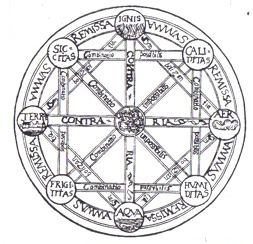
\includegraphics[scale=0.9]{images/characteristica_universalis_diagram.jpg}
\caption{Leibniz's diagrammatic reasoning in ``Dissertatio de arte combinatoria''}
\end{figure}

\newpage
While these first forays into the subject solely wanted a language for scholars, more ambitious plans for an artificial language that all nations and people could use came soon after,
with scepticism from several authors. An example of such disagreement can be found in some of Descartes' letters exchanged with fellow polymath Marin Mersenne (in 1629), the former
stating that he does not see any use for such a language, but if it were to exist it would require several aspects:

\begin{itemize}
    \setlength\itemsep{-0.5em}
    \item be international;
    \item outlined by a simple grammar, that could be learned in a few hours;
    \item possess neither exceptions nor irregularities. \footcite[76-82]{descartes1897oeuvres}
\end{itemize}

The disagreement notwithstanding, Mersenne eventually created his own ``universal language for research'', that he presented in his 1636 book
``Harmonie universelle, contenant la th{\'e}orie et la pratique de la musique'', containing a proposal for a ``perfect language'', expressing scientific
concepts through music. \footcite[Book I, proposition 24]{mersenne1636}

\section{Constructed languages}

The criteria defined by Descartes are still today the baseline that a lot of authors use for the definition of what an optimal language should be, and are at the core of many
constructed languages. These languages are the artificial counterpart to natural languages: while the latter are the the unconscious natural evolution of existing languages through
time, the grammar, vocabulary, writing system, and other linguistic elements of constructed languages were fully devised from scratch by one or more people. Important note
however --- through use, these constructed languages can also potentially evolve with time, but it is a conscious effort brought forth by its users, and not the effect of human
trends in the language.\newline

Constructed languages are usually divided into three groups, based on their purpose:\newline

\textbf{Auxiliary languages}: this group of languages aims to serve as a secondary language for people all around the world to communicate seamlessly.
They serve as a sort of ``lingua franca'', but without the usual factor of dominance associated to them (socio-economic or political). Some of them have a secondary social aim:
bridge cultures and countries in order to bring peace to the world. Notable examples of languages in this category are Esperanto, Volapük, Ido, and Interlingua.

\textbf{Artistic languages}: group of languages designed as artistic projects, or ways to expand works of fiction and give them more depth. Notable examples of languages
in this category come from many different mediums, such as books (Sindarin and Quenya --- Lord of the Rings, Newspeak --- Nineteen Eighty-Four, and  Nadsat --- A Clockwork Orange),
TV shows (Klingon --- Star Trek, Valyrian and Dothraki --- Game of Thrones, and Goa'uld --- Stargate) or even comic books (Syldavian --- Tintin).

\textbf{Engineered languages}: languages created in order to explore theories in the field of linguistics. Notable examples of languages in this category are Loglan, Lojban, and Toki Pona\newline

A second method of classification for constructed languages was devised in 1903 by Louis Couturat and Léopold Leau
in ``Histoire de la langue universelle''\footcite[Introduction, Pages XXVII and XXVIII]{couturat1903histoire}:

\begin{itemize}
    \setlength\itemsep{-0.5em}
    \item A priori system: language whose features are not based on an existing language --- often introducing brand new writing systems, invented grammar structures,
    or a taxonomy for words and concepts;
    \item A posteriori system: language whose features are based in one or several existing languages --- many of which are often criticized for being ethnocentric, and
    creating auxiliary languages that draw inspiration from mostly European countries, which defeats the purpose of an all encompassing world-wide language;
    \item Mixed system: when the language has features that fall into both systems.
\end{itemize}

All these classifications are of course loose definitions: a language may fall under more than one category in terms of purpose, for example. For an in-depth history of
constructed languages, I recommend the reader to explore Arika Okrent's book \footcite{okrent2009land}. While it is not a scientific publication, it is an extremely
comprehensive and rich book to dive deep into the subject.\newline

\vspace{-0.05cm}
Albeit still being a niche subject, these languages have grown in popularity in the last few years. Following Esperanto, a few of them have risen to the eyes of the public
given their origins. Most of these languages could be classified in the ``artistic languages'' group, as they originate from works of fiction. Due to the popularity of those works of
fiction, the general public is being exposed to the concept of constructed languages. The most notable example of this growth in popularity is the language learning platform
``Duolingo'' introducing courses for three of them: Esperanto, High Valyrian (invented for the TV show ``Game of Thrones'') and Klingon (invented for the TV show ``Star Trek''). \newline

\vspace{-0.05cm}
Unfortunately, due to the notable difference in popularity between Esperanto and other such languages, research in the field of linguistics has mostly been focused on the former.
This focus is understandable: Esperanto is one of the few constructed languages that can boast having native speakers. Detlev Blanke highlights this achievement, putting Esperanto
in a category of its own as a full-fledged language, and not a ``language project'' or a ``semilanguage''. He theorises that it is the only constructed language that has gone through nineteen
evolutionary steps he describes, ``from the publication of its structure to the appearance of the first bilingual children'' \footcite{blanke1989planned}.
Since the publication of his article, Klingon can probably claim the same status, but researchers probably don't delve into it as much due to its origins.
Nonetheless, authors have been urging researchers to study other constructed languages, as these may have troves of interesting linguistic elements \footcite{oostendorp2001constructed}.

\section{Lojban}

\subsection{The roots: the history of Loglan}

The first constructed language whose main aim is optimality is most probably Loglan, introduced by James Cooke Brown and first published
in Scientific American \footcite{brown1960loglan}. This is a notable achievement: rarely had a major scientific periodical devoted publishing
space to a constructed language other than Esperanto. This is probably due to the fact that Brown presented it with a purely scientific approach, and no big societal aims
(at first --- history will change that). Loglan, whose name is a contraction of the words ``Logical'' and ``Language'', was defined as having the following aims:

\begin{itemize}
    \setlength\itemsep{-0.5em}
    \item be purely based in logic;
    \item be culturally neutral;
    \item have a grammar small enough to be teachable, but complex enough to allow conversations;
    \item be unambiguous.
 \end{itemize}

The history of Loglan will take a strange path after its first publication. Given its publication in a major scientific journal, and a growing audience
asking him for more information, Brown requested a raise from his university, which was declined, and a government grant, which was also refused multiple times.
Insulted, he eventually resigned from his research position and, using money gathered by activities other than scientific research, started his own institute,
the ``Loglan Institute''. Later, in 1975, he published a book about the language. At the institute, he surrounded himself mostly by admirers, most of which were computer science
students and researchers who were excited by the possibility of the language serving as a human-computer interface. Thus, Brown rarely opened himself to critics,
which might have influenced the inflated sense of importance he felt Loglan had. A less explicit aim for the language, that was presented at a later point, was attempting
to prove the hypothesis of linguistic relativity (also known as the Sapir–Whorf hypothesis, or simply the Whorf hypothesis) in its strong version.
Most modern linguists would disagree with this statement, but Brown was convinced that the usage of Loglan would allow speakers to think more logically, and expand their
intelligence.\newline

With a growing audience, and the transformation of the institution into a ``membership-controlled corporation'' (in order to request paying fees to all the volunteers),
Brown started to see that its members wanted to steer his creation in a direction he did not enjoy. Trying to remain in control, he fired most of the board.
This event and others created a schism in the Loglan community, and little by little a separatist group grew, which gave birth to Lojban.

\subsection{The creation of Lojban}

Starting in 1987, The Logical Language Group (LLG) worked to create a constructed language that aimed to extend the existing Loglan language and improve it further,
in order to make it easier to learn by humans and more readily accessible. This work culminated with the publication of a book in 1997 by
John Woldemar Conwan \footcite{cowan1997complete}, an American programmer otherwise known for his work with XML and Unicode, among other things. This book is,
still today, considered the baseline of the language, defining its whole grammar, vocabulary, and semantics.\newline

Over the years, Brown disputed several times in court that this creation infringed his copyright. Several trials later, all courts agree that both projects
are independent, and Lojban took over Loglan in popularity and contributors.\\

Lojban claims to be a syntactically unambiguous language that improves human-human communication but also human-computer
communication. While the former is more complicated to prove, since the amount of speakers of Lojban around the world is not immense,
the latter has been studied. Research has already postulated that Lojban (or variants of it) would be interesting interlinguas between
humans and computers \footcite{speer2004meeting} or artificial intelligences \footcite{goertzel2013lojban}.

\subsection{(Very) Brief introduction to the Lojban grammar}
\label{subsec:brief-intro-to-lojban}

Lojban sentences are constructed in a way that expresses a logical predicate, with a fixed set of arguments.
The recurring ``first approach to the language'' example used in most Lojban literature, from the language standard
to research papers is the sentence ``John is the father of Sam''. In this sentence, there is a clear predicate
(``is-the-father-of'') and two arguments (``John'' and ``Sam'').

\begin{figure}[H]
\centering
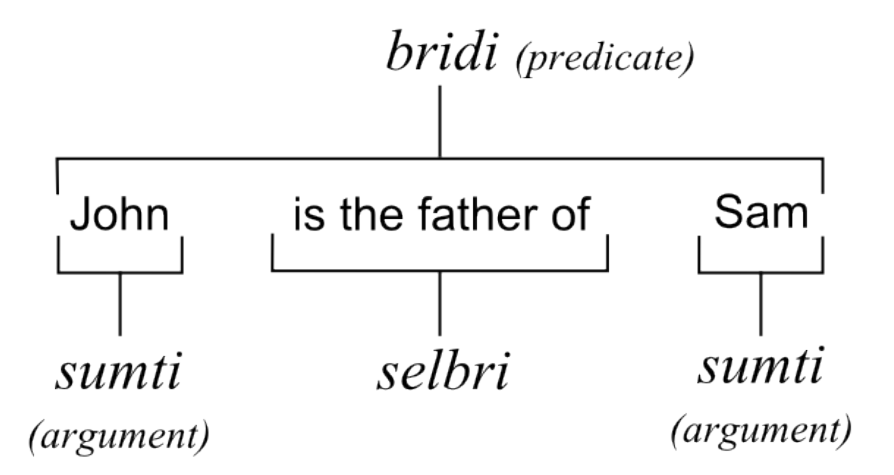
\includegraphics[scale=0.20]{images/lojban_grammar.png}
\caption{Basic structure of a Lojban sentence (Source: \cite{cowan1997complete})}
\end{figure}

This figure presents the three most important base elements of a sentence in Lojban:

\begin{itemize}
    \item \textbf{bridi}: the predicate expression;
    \item \textbf{selbri}: the word(s) acting as the predicate;
    \item \textbf{sumti}: positional argument passed to the predicate.
\end{itemize}

Selbri are strictly defined by representations which position the sumti around a key word. For example, the selbri to describe the fatherhood relationship is ``patfu'':

$$\text{patfu}: x_1 \: \text{is a father of} \: x_2$$

Thus, the above sentence is expressed in Lojban as: \textbf{la .djon. patfu la .sam.} \newline

If no modifiers are used, the position of the sumti is rigid and allows to release the sentence from any ambiguity. We always know who is the father and who is the child.
Of course, in this example, the English counterpart doesn't really make sense (the sentence ``Sam is `fathered' by John'' makes absolutely no sense), but for a non-native speaker
the order of words in other pairs of sentences might add ambiguity.\\

For example, a non-native English speaker might get confused about the difference between the sentences ``My dog bites the man''
(\textbf{``le mi gerku cu batci le nanmu''} in Lojban) and ``The man is being bitten by my dog'', as this inverted construct might not exist in their language.
Lojban solves this issue by having a specific keyword, indicating that two or more sumti (positional arguments) are going to be swapped. This allows speakers, even those not
familiar with this grammatical construct, to understand the difference between two very different sentence constructions: e.g. ``The man is being bitten by my dog''
and ``The man is biting my dog''.\newline

Of course, this framework of predicate expressions is simply the base feature of the language, but many others allow it to cover the other missing aspects that most natural
languages feature: tenses, relative clauses, abstractions, emotional indicators, and many others. These will be explored further in Part \ref{part:creating-a-peg} of this thesis. \newline

Another very interesting aspect of Lojban is its creators will to avoid one big flaw many other "a posteriori" constructed languages have: being
eurocentric and drawing inspiration from European languages only. All core verbs were created by taking the corresponding words in the six languages most spoken
in the world at that time (Chinese, Hindi, English, Spanish, Russian and Arabic, ranked by number of speakers), transformed to fit Lojban's morphological rules,
and given a score by an algorithm. After handling possible collisions with existing words, and other minute grammatical rules, Lojban's core vocabulary
was created, and continues to be enriched with the same algorithm today (with some changes to the scoring being done due to demographic changes in the world).

\subsection{Learning Lojban}
\label{subsec:learning-lojban}

TODO

Vaguely: it's super complicated, many advanced references (namely THE book),
\chapter{Aims and objectives of this thesis}

\vspace{0.5cm}

At its root, computer science had a singular aim --- automating calculations for a broad spectrum of use-cases.
However with time and with the emergence of better, faster, and stronger computers, researchers understood that computers could be used to achieve
far more complex tasks. Several diverse research fields made their appearance, and among these some realised that computing could help us structure the
flow of information, in addition to making calculations based on it. \newline

The explosion of tasks requiring the processing of large amounts of structured data inside of companies, and much later the arrival of the Internet,
forced us to debate and research subjects such as: how to gather information, how to manage and store it, analyse and interpret it, explore it, etc...
A sizeable chunk of this information comes to us in the form of text and language, in their many forms. To answer these needs, language engineering became a
central research field in a new society, one that had migrated from a purely industrial society to an ``information society''.\newline

This thesis aims to accompany the reader through the exploration of the intersection between two fields: linguistics (constructed languages)
and computer science (language processing, parsing expression grammars, and others). Lojban, being a language purely based in logic, seems like a very
interesting candidate to help us through this exploration. Unfortunately, as seen in \ref{subsec:learning-lojban}, Lojban is not an easy language to study.
What if learners had a set of tools which helped them understand Lojban's grammar, through analysis and visualisation of parsed sentences?
This thesis aims to create such a set of tools.\newline

\newpage

To do so, some objectives are needed. They are the following:
\begin{itemize}
\item Outline the state of the art and existing tools/resources for Lojban (Part \ref{part:state-of-the-art})
\item Create tools, written in the Python programming language, to explore Lojban sentences and help learners of this
language to understand how it is structured (Part \ref{part:python-toolkit})
\item Create a simplified Parsing Expression Grammar (PEG) for Lojban, used by the tools created,
which allows the reader to learn the basics of Lojban's grammar while reading a set of parsing expressions (Part \ref{part:creating-a-peg})
\item Examine if these objectives were met, and outline future work (Part \ref{part:conclusion})
\end{itemize}
\newpage \thispagestyle{empty} \ \newpage
% Part 2
\part{State of the art}
\label{part:state-of-the-art}
\chapter{Existing research and references}

\newpage \thispagestyle{empty} \ \newpage

\chapter{Existing resources and tools for Lojban}
\label{chap:existing-resources-and-tools}

\vspace{0.5cm}

\section*{Grammars}
\label{section:lojban-grammars}

Camxes

https://mw.lojban.org/papri/camxes

Java

Camxes.js

http://masatohagiwara.net/camxes.js/

javascript

La ilmentufa

https://mw.lojban.org/papri/la\_ilmentufa


\section*{Parsers}

Official LLG Parser

https://mw.lojban.org/papri/Official\_LLG\_Parser

C78 source code
or
MS-DOS executable

\begin{itemize}
    \item BPFK Parser: official parser for Lojban maintained by the Logical Language Group (LLG) - implements the official grammar and is intended to be the reference parser for the language.
    \item jlöi parser
    \item plise parser
    \item Lojban Natural Language Toolkit (LONU)
    \item Zantufa
    \item lojban-parsing
\end{itemize}

\section*{Dictionary}
\label{sec:dictionary}

jbovlaste is the Lojban dictionary. \\

la sutysisku, interface for la jbovlaste database with some algorithms improving search relevance. \\

Lojban Online Dictionary Query. The jbovlaste search engine.\\
\newpage \thispagestyle{empty} \ \newpage
% Part 4
\part{Creating a Python-Lojban toolkit}
\label{part:python-toolkit}
\chapter{Introduction}
\chapter{Defining words: the ``dictionary'' module}
\label{chap:creating_a_dictionary}

\section{Methodology}

Described in \ref{sec:dictionary}, La Jbovlaste is the official Lojban dictionary published by the LLG and available online \footcite{jbovlaste}.
This dictionary allows to export the entirety of its data in a XML format at the "XML Export" page \footcite{jbovlaste-export}.\\

\newpage

The format of the XML file is as follows (showing the example of a single word, jbovlaste itself): \\

\begin{lstlisting}
<?xml version="1.0" encoding="UTF-8"?>
<?xml-stylesheet type="text/xsl" href="jbovlaste.xsl"?>
<dictionary>
  <direction from="lojban" to="English">
    (...)
    <valsi word="jbovlaste" type="lujvo">
      <user>
        <username>djeikyb</username>
        <realname>Jacob Thomas Errington</realname>
      </user>
      <definition>$x_1=li_1$ is a list of words $x_2=v_1$ in Lojban ($v_3$=lo lojbo), in order $x_3=li_3$, preserved in medium $x_4=li_4$.</definition>
      <definitionid>32240</definitionid>
      <notes>In a la-description, jbovlaste refers to the online dictionary editing system.</notes>
      <glossword word="dictionary" sense="lojban word list" />
    </valsi>
    (...)
  </direction>
</dictionary>
\end{lstlisting}

\section{Examples of usage}

\begin{lstlisting}
  >>> from dictionary.jbovlaste import Jbovlaste
  >>> jbovlaste = Jbovlaste()
  >>> for key, values in jbovlaste.get_whole_dict().items():
  ...     print(key, len(values))
  ...
  cmavo 598
  cmavo-compound 607
  fu'ivla 3901
  experimental cmavo 856
  cmevla 481
  obsolete fu'ivla 302
  bu-letteral 36
  zei-lujvo 147
  lujvo 7388
  experimental gismu 306
  gismu 1342
  obsolete cmevla 28
  obsolete cmavo 2
  obsolete zei-lujvo 3
  >>>
  \end{lstlisting}

\section{Breakdown of the code produced}

The code produced is found at Annex \ref{appendix:jbovlaste-annex}

\subsection{\_\_init\_\_.py file}

Allows other modules to import the Jbovlaste class without calling the file it is contained in explicitly.

\subsection{jbovlaste.py file}


\chapter{The ``grammar\_parser'' module}

\section{Methodology}

\section{Parsing Lojban sentences}
\label{sec:parsing_lojban_sentences}

Described in Subsection \ref{sub:parser}.

\lstinputlisting[language=Python]{./code/grammar_parser/gentufa.py}

(See Appendix \ref{appendix:gentufa-annex} for the corresponding annex)

TODO
\chapter{Creating a test suite: the "tests" folder}
\label{chap:creating_a_test_suite}

\section{Methodology}

Writing a Parsing Expression Grammar (see next part of the thesis) requires constant vigilance in order to make sure
that any rule change doesn't impact several nodes of the grammar at the same time, thus breaking its parse tree. Running test
sentences one by one, by hand, would be time consuming and not very scientific (especially if there are hundreds of test sentences).\newline

In order to evaluate scientifically the validity and degree of completeness of the code and grammar produced, a test suite must be created.
Additionally, a data set with enough sentences to evaluate is required. Thankfully, throughout the chapters of \citetitle{cowan1997complete},
\citeauthor{cowan1997complete} gives us a trove of example sentences.\newline

Using the PyTest Python library \footcite{pytest8.3.2}, a test suite will be constructed in order to run the "grammar\_parser" module
and the "visitor" module on all sentences collected.

\section{Breakdown of the folder}

The code produced is found at Annex \ref{appendix:parser-testing-annex}. You may read it along the following explanations.

\newpage

\subsection*{conftest.py file}

This file has two functions: \newline

The \textbf{sentences} function lists all files present in the "sentences" folder and opens them one by one,
in order to collect the test sentences. For each sentence, we also list what chapter it comes from (through the file name) and
at what line in the test file it located at.\newline

The \textbf{build\_test\_parameters} function uses the previous function as a PyTest fixture, in order to yield the test sentences and
their context one by one to the actual test function, found in the next file.

\subsection*{test\_gentufa\_and\_visitor.py file}

In this file, outside of the test function, an instance of the Gentufa class is created, which will be used to parse all test sentences.\newline

The test function, called \textbf{test\_chapter\_sentences}, receives the sentences one by one thanks to the \textbf{build\_test\_parameters} function
described above. For each sentence, we first run the parser, marking the test as a failure if the parser returns an exception (either IncompleteParseError
or ParseError). Then, the parse tree generated is fed to an instance of the GentufaVisitor class, and we check if the "visit" worked fine and if the output
has a valid format. If an exception was raised (either VisitationError or TypeError), we mark the test as a failure.

\subsection*{sentences directory}

The "sentences" directory contains many files, one per chapter, listing all the sentences which will compose the dataset.
All test sentences are surrounded by comments giving context about which chapter and section of the book they come from.

\newpage

\begin{lstlisting}[caption=Example of a test file with some sentences to be parsed]
### Chapter 2.5 ###
# Example 2.11
mi tavla do zo'e zo'e
# Example 2.12
do tavla mi ta zo'e
# Example 2.13
mi tavla zo'e tu ti
# Example 2.14
mi tavla do
# Example 2.15
do tavla mi ta
\end{lstlisting}

\newpage

\section{Examples of usage}

The test suite is run by executing a makefile at the root of the code directory with the following command: \textbf{make tests}.
Once executed, all tests will run and a test run summary is displayed. There are two possible outcomes: either all tests pass correctly,
or errors have been introduced. \newline

Thankfully, due to proper error-handling and test cases management, the test suite outputs for each error:

\begin{itemize}
    \item what sentence the error corresponds to, which file it comes from, and at which line it is in the file (which is useful due to the
    added context given in the test files which was explained previously)
    \item whether it was the Parser class that failed, or the Visitor class
    \item above the test run summary each error is displayed with a traceback, which thanks to Parsimonious' \footcite{parsimonious} good error
    handling highlights explicitly which part of the grammar or the visitor is failing.
\end{itemize}

This is extremely useful in order to debug at which layer the error was introduced. \newline

The following figures display examples of these two possible outcomes:\newline

\begin{figure}[H]
\hspace{-1.1cm}
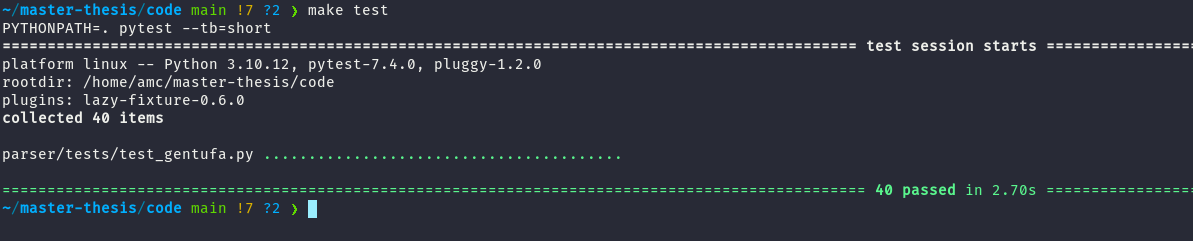
\includegraphics[scale=0.43]{images/pytest_output_pass.png}
\caption{Pytest Output Example - All tests passing}
\end{figure}

\begin{figure}[H]
\hspace{-1.8cm}
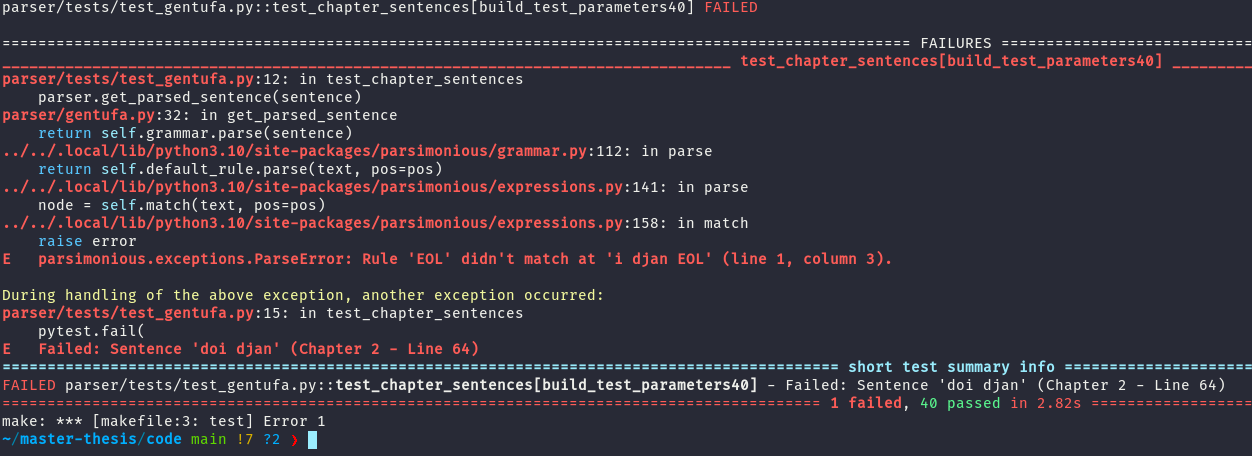
\includegraphics[scale=0.30]{images/pytest_output_fail.png}
\caption{Pytest Output Example - An error occured}
\end{figure}
% Part 3
\part{Creating an ``educational'' PEG for Lojban}
\label{part:creating-a-peg}
\chapter{Introduction}

\vspace{0.5cm}

As seen in Chapter \ref{chap:existing-resources-and-tools}, the existing formal grammars for Lojban are extremely complete.
They cover the entirety of the language, both in its morphology and syntax/semantics, which means they can even validate words that don't exist yet
as long as they fit the language's rules (as mentioned in \ref{subsec:brief-intro-to-lojban}, an algorithm for "word creation" exists).
However, this completion makes these formal grammars extremely complex to read for a beginner, and are simply tools to be used by machines. \newline

As an example, here is an extract of the first few "root nodes" of GRAMMAR NAME: \newline

ADD EXTRACT OF GRAMMAR HERE \newline

What if there existed a formal grammar which people could read along, while learning Lojban, in order to gather a deeper
understanding of the language? For any other language, using a formal grammar file as a learning companion would be a very obscure method.
However, Lojban being a language that can be parsed just as a programming language would, it would be very interesting to build a formal grammar
which would help a prospective student understand the intrinsic rules behind the language's grammar. \newline

Of course, improving the reading comprehension of a formal grammar reduces the complete aspect of it:

\begin{itemize}
  \item It is almost impossible to address all rules of the grammar, as some of them are extremely complex;
  \item Ignoring the morphology of words means that unknown but valid words won't be accepted;
\end{itemize}

However, as a beginner's tool, such a grammar could really improve the steep learning curve of Lojban, in my opinion.\newline

The next chapter will explore the main reference for Lojban (\cite{cowan1997complete}), in its 2016 revised version, and write a simplified parsing expression grammar (PEG) for a subset of the language.

% https://en.wikipedia.org/wiki/Extended_Backus%E2%80%93Naur_form

% https://en.wikipedia.org/wiki/Parsing_expression_grammar
\chapter{Learning Lojban by writing a PEG}

\section{Creating a test suite}
\label{sub:creating_a_test_suite}

(See Appendix \ref{appendix:parser-testing-annex} for the corresponding annex)

\begin{figure}[H]
\hspace{-1.1cm}
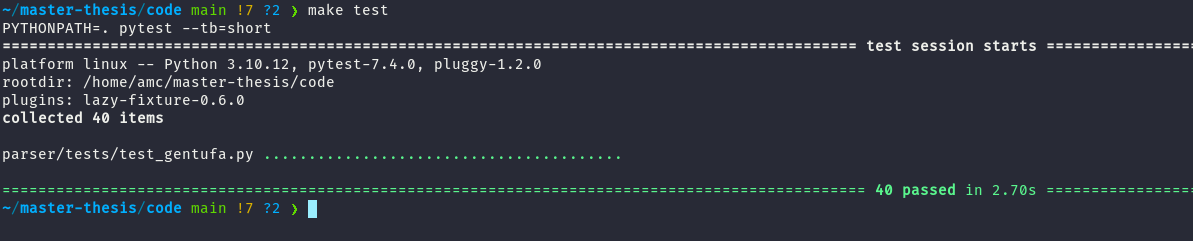
\includegraphics[scale=0.43]{images/pytest_output_pass.png}
\caption{Pytest Output Example - All tests passing}
\end{figure}

\begin{figure}[H]
\hspace{-2.2cm}
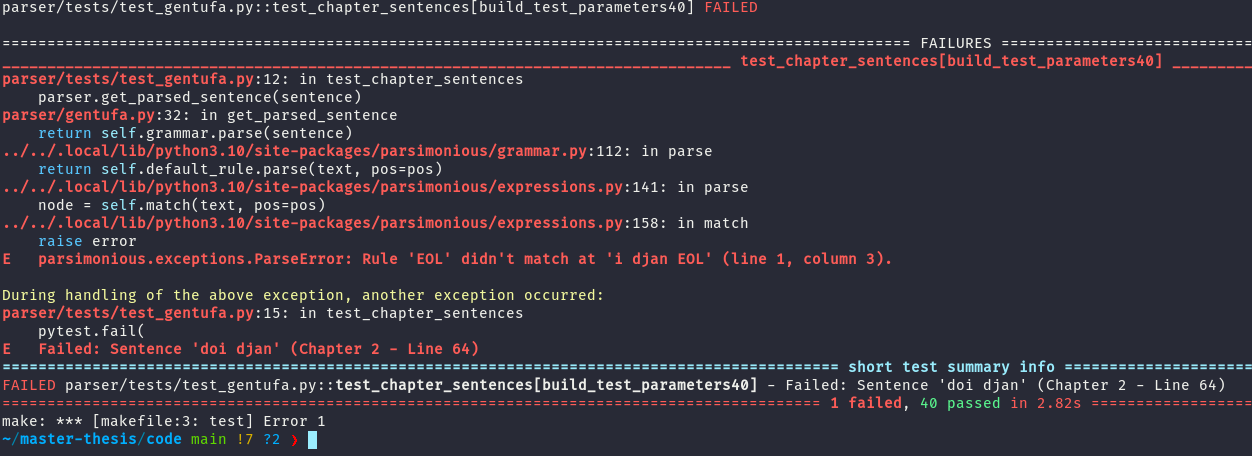
\includegraphics[scale=0.43]{images/pytest_output_fail.png}
\caption{Pytest Output Example - Error}
\end{figure}
\part{Visualising parsed sentences}
\label{part:visitor-and-visualising}
\chapter{Tagging and labeling parsed sentences: the ``visitor'' module}
\label{chap:visitor-module}

\section{Methodology}

Parsimonious has the visitor function. Allows to explore the parse tree generated

What we achieve is a mix of Parts-Of-Speech tagging (giving each word a grammatical category) and Semantic role labeling
because tagging verbs allows us, thanks to their definition, to know which word accomplishes what role in the sentence.

% https://www.geeksforgeeks.org/nlp-part-of-speech-default-tagging/

% https://en.wikipedia.org/wiki/Semantic_role_labeling

\section{Breakdown of the module}
\label{sec:visitor-code-breakdown}

The code produced is found at Annex \ref{appendix:gentufa-visitor-annex}.

TODO

\newpage

\section{Examples of usage}

This module can be used in two different ways: as a command-line interface (CLI) tool
from a terminal, or as a class for short scripts or other modules to use.

\begin{lstlisting}[caption=GentufaVisitor module being used as a command-line interface tool]
$ python3 visitor/gentufa_visitor.py "mi klama le zarci" | jq

{
  "sentence": "mi klama le zarci",
  "segments": [
    {
      "mi": {
        "definition": "I/me, we/us",
        "type": "cmavo / KOhA selma'o (mi series) / pronoun"
      }
    },
    {
      "klama": {
        "definition": "$x_{1}$ comes/goes to destination $x_{2}$ from origin $x_{3}$ via route $x_{4}$ using means/vehicle $x_{5}$.",
        "glosswords": [ {"word": "come", "sense": null} ],
        "type": "gismu",
        "sumti": [ "$x_{1}$", "$x_{2}$", "$x_{3}$", "$x_{4}$", "$x_{5}$" ]
      }
    },
    {
      "le zarci": {
        "type": "description brivla",
        "segments": [
          {
            "le": {
              "definition": "description marker / 'the'",
              "type": "cmavo / LE selma'o"
            }
          },
          {
            "zarci": {
              "definition": "$x_{1}$ is a market/store/exchange/shop(s) selling/trading (for) $x_{2}$, operated by/with participants $x_{3}$.",
              "glosswords": [
                { "word": "market", "sense": null },
                { "word": "shop", "sense": "store" }
              ],
              "type": "gismu",
              "sumti": [ "$x_{1}$", "$x_{2}$", "$x_{3}$" ]
            }
          }
        ]
      }
    }
  ]
}
\end{lstlisting}

\newpage

\begin{lstlisting}[caption=GentufaVisitor class being used by a Python script]
>>> from grammar_parser import Gentufa
>>> from visitor import GentufaVisitor
>>> parse_tree = Gentufa().get_parsed_text("mi klama le zarci")
>>> visitor = GentufaVisitor(parse_tree)
>>> visitor.get_json_output()
'{"sentence": "mi klama le zarci", "segments": [{"mi": {"definition": "I/me, we/us", "type": "cmavo / KOhA selma\'o (mi series) / pronoun"}}, {"klama": {"definition": "$x_{1}$ comes/goes to destination $x_{2}$ from origin $x_{3}$ via route $x_{4}$ using means/vehicle $x_{5}$.", "glosswords": [{"word": "come", "sense": null}], "type": "gismu", "sumti": ["$x_{1}$", "$x_{2}$", "$x_{3}$", "$x_{4}$", "$x_{5}$"]}}, {"le zarci": {"type": "description brivla", "segments": [{"le": {"definition": "description marker / \'the\'", "type": "cmavo / LE selma\'o"}}, {"zarci": {"definition": "$x_{1}$ is a market/store/exchange/shop(s) selling/trading (for) $x_{2}$, operated by/with participants $x_{3}$.", "glosswords": [{"word": "market", "sense": null}, {"word": "shop", "sense": "store"}], "type": "gismu", "sumti": ["$x_{1}$", "$x_{2}$", "$x_{3}$"]}}]}}]}'
\end{lstlisting}
\chapter{Visualising a broken down sentence: the "visualize" module}

% Compare to https://la-lojban.github.io/parser/#q=mi_tavla_do&l=dagreH&c=compact-all
\newpage \thispagestyle{empty} \ \newpage
% Part 5
\part{Conclusion}
\label{part:conclusion}
\chapter{Future work}

\vspace{0.5cm}

Future work

- Visualisation module
- Address more aspects of the grammar
- Improve "visitor" functions in order to be more generic and avoid having to
create functions for ALL nodes of the Parse Tree, which is frustrating.
\chapter{Results and closing remarks}

\vspace{0.5cm}

The conjunction of the parser, the visitor, and the PEG created in this thesis currently cover most of the language described in
\citetitle{cowan1997complete} until chapter 7 (with a few excursions into other chapters). 21 chapters exist in the book,
but only 17 chapters that address grammar, which means that this thesis achieved to create tools which help students of
Lojban to understand more than 40\% of the major reference book on the language. \newline

The final test coverage is as follows:

\begin{itemize}
    \item 200 sentences from 7 chapters were selected;
    \item of these 200 sentences, 186 were parsed and visited correctly;
    \item thus the apparent success rate of the parser, for this dataset is 93\%
\end{itemize}

However, it is important to note that Chapter 2 of the reference book gives a very broad tour of the language, so the tools
developed allow true beginner students to study in depth the most important chapter of all.\newline

Looking back at the aims and objectives set in Chapter \ref{chap:aims-and-objectives}, one must ponder if they were met. Let us
revisit them and evaluate:

\begin{itemize}
\item \textbf{State of the Art (Part \ref{part:state-of-the-art})}: A broad overview of the study of constructed languages, and Lojban
in specific, was created in order to gain deeper understanding on the subject.
\item \textbf{Creation of a Python-Lojban toolkit (Part \ref{part:python-toolkit})}: Three different tools were created, each
serving a separate purpose but working in collaboration. These tools allow students, while learning Lojban, to gather word definitions,
test if the sentences they are writing are correct, and decompose complex sentences they might struggle to understand.
\item \textbf{Creation of a simplified Lojban PEG (Part \ref{part:creating-a-peg})}: The created grammar is, of course, not complete.
Several grammar aspects are still missing, it over-simplifies some of the rules, and possibly validates sentences that other parsers wouldn't.
However, while creating it, I was able to understand Lojban much better than with the few tutorials existing online, which means that this way
of studying (reference book + companion grammar) does have at least some anecdotal success. The only way to assess the veracity of this point
would be to convince people to study Lojban and do a parallel study.
\end{itemize}

The overarching objective was to create a learning companion for students. It is fair to say that at least this humble objective was met,
and that these tools are a good starting point for continued work in the subject.\newline

Learning a language is never easy, and for one as complex as Lojban this expression is an understatement. As someone who has always been interested
in (self-)education, I hope that the work accomplished in this thesis, and the future work planned ahead, might help prospective
learners of Lojban one day.

% Bibliography
\nocite{*}
\makeatletter
\@openrightfalse
\makeatother
\part*{Bibliography}
\addcontentsline{toc}{part}{Bibliography}
\pagestyle{fancy}
\newgeometry{left=2cm}
\printbibliography[
    category=cited,
    heading=subbibliography,
    %title={Bibliography},
    resetnumbers
]
\newpage
\printbibliography[
    notcategory=cited,
    heading=subbibliography,
    title={Not cited yet},
    resetnumbers
]

% Appendices
\makeatletter
\@openrightfalse
\makeatother
\pagestyle{empty}
\part*{Appendices}
\addcontentsline{toc}{part}{Appendices}
\appendix
\newgeometry{left=1.8cm, right=0.5cm, top=1.5cm, bottom=1.5cm}
\chapter{Code produced for this thesis}

\section{Jbovlaste}
\label{appendix:jbovlaste-annex}

Described in Subsection \ref{sub:creating_a_dictionary}.

\lstinputlisting[language=Python]{./code/dictionary/jbovlaste.py}

\newpage

\section{Test Suite}
\label{appendix:test_suite}

Described in Subsection \ref{sub:creating_a_test_suite}.

\lstinputlisting[language=Python]{./code/parser/tests/test_gentufa.py}

\newpage

\section{PEG}
\label{appendix:peg-annex}

Described in Subsection \ref{sub:peg}.

\lstinputlisting{./code/parser/gerna.peg}

\newpage

\section{Gentufa}
\label{appendix:gentufa-annex}

Described in Subsection \ref{sub:parser}.

\lstinputlisting[language=Python]{./code/parser/gentufa.py}


\newpage \ \newpage

\end{document}